\section{Criação dos \textit{datasets}}
\label{sec:metodos-datasets}

O primeiro passo para desenvolver e avaliar a abordagem proposta consiste em estabelecer um \textit{dataset} que viabilize essa forma de modelar o problema. Como a proposta apresentada aqui é nova, não existem \textit{datasets} diretamente compatíveis com ela e, por este motivo, será derivado um novo a partir de outro já existente -- o \acrfull{asllvd}.

O \acrshort{asllvd}~\cite{athitsos-2008-asllvd,neidle-2012-asllvd} é um \textit{dataset} público\footnote{Disponível em \url{http://www.bu.edu/asllrp/av/dai-asllvd.html}} amplo da \acrshort{asl} que contém aproximadamente 2.745 sinais representados em cerca de 9.763 sequências de vídeo. Esses sinais são articulados por indivíduos Surdos nativos na língua e foram capturados por meio de quatro câmeras distintas sincronizadas: uma visão frontal em alta resolução a meia velocidade, outra visão frontal, uma visão lateral e uma visão da face, conforme ilustrado na \autoref{fig:asllvd-example}.

\begin{figure}[ht!]
    \centering
    \caption{\textmd{Exemplo de três perspectivas capturadas pelo \acrshort{asllvd} para o sinal MERRY-GO-ROUND}}
    \borda[0.85\textwidth]{
        \subcaptionbox{Vista frontal \label{subfig:asllvd-example-front}}{
            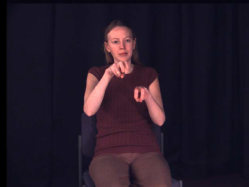
\includegraphics[height=3cm]{capitulos/metodos/imagens/asllvd_example_front}
        }%
        \hfill
        \subcaptionbox{Vista lateral \label{subfig:asllvd-example-side}}{
            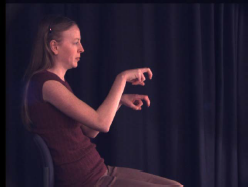
\includegraphics[height=3cm]{capitulos/metodos/imagens/asllvd_example_side}
        }%
        \hfill
        \subcaptionbox{Vista da face \label{subfig:asllvd-example-close}}{
            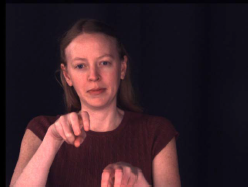
\includegraphics[height=3cm]{capitulos/metodos/imagens/asllvd_example_close}
        }%
    }
    \nomefonte[p. 2]{athitsos-2008-asllvd}
    \label{fig:asllvd-example}
\end{figure}


Para que fosse possível extrair \textit{features} no formato de parâmetros fonológicos a partir das amostras do \acrshort{asllvd}, que são compostas essencialmente de sequências de vídeos com \textit{frames} em RGB, foi necessário realizar um processo em duas etapas.

Na primeira, foi realizada a estimativa das coordenadas dos esqueletos dos indivíduos de cada \textit{frame} para duas das perspectivas fornecidas para as amostras, os quais foram combinados em seguida para compor um esqueleto tridimensional final. A saída dessa etapa deu origem ao \textit{dataset} intermediário denominado ASL-Skeleton3D.
Na segunda etapa, foi aplicado um conjunto de operações algébricas sob esse esqueleto tridimensional para finalmente computar os parâmetros fonológicos, processo esse que originou o \textit{dataset} ASL-Phono.


Esse processo de extração de \textit{features} envolveu alguns desafios relevantes, dentre os quais podem-se enumerar:

\begin{enumerate}
    \item Definição de uma estratégia para representar indivíduos no espaço tridimensional utilizando apenas \textit{frames} de vídeo bidimensionais simples, bem como para contornar a ausência de perspectivas ou a baixa qualidade de algumas dessas amostras;

    \item Estabelecimento de um subconjunto inicial de atributos fonológicos capaz de capturar e representar variações significativas na articulação dos sinais, e que ao mesmo tempo pudessem ser modelados computacionalmente nessa primeira iteração da abordagem proposta.

    \item Identificação de técnicas matemáticas e medidas antropométricas que pudessem fundamentar a modelagem e o cálculo desses atributos.

    \item Demanda por recursos computacionais significativos para processar duas perspectivas distintas para cada uma das quase 10.000 amostras contidas em cada \textit{dataset}. Em média, isso consumiu cerca de 120 horas contínuas de processamento distribuído com GPUs e gerou mais de 1 TB de dados cada vez que os \textit{datasets} precisaram ser gerados novamente.
\end{enumerate}


% Dataset 3d
\subsection{ASL-Skeleton3D}
\label{sec:metodos-datasets-3d}

%FIXME: [cz] como é uma contribuição relevante do seu trabalho eu acho que isso deveria ser uma seção nova

O ASL-Skeleton3D é um \textit{dataset} intermediário que introduz a representação em coordenadas 3D das amostras do \acrshort{asllvd}. 
Esse tipo de informação fornece detalhes mais precisos acerca do corpo dos indivíduos enquanto eles articulam os sinais, o que possibilita a pesquisadores em \acrshort{slr} extrair diferentes tipos de \textit{features}, explorar novas técnicas, ou ainda derivar outros novos \textit{datasets}.
Além disso, essa representação é genérica e pode ser replicada para outras línguas de sinais.
% %FIXME [cz] Importante enfatizar que as representações propostas são genéricas e podem servir como base para qualquer linguagem de sinais. --> [cca5] feito

Para que fosse possível projetar as amostras do \acrshort{asllvd} dentro do espaço tridimensional, adotamos uma estratégia que consiste em combinar duas perspectivas 2D perpendiculares entre si -- a vista frontal e a vista lateral -- para reconstruir uma perspectiva 3D, conforme ilustra a \autoref{fig:our-strategy-3d}. Com isso, assumimos que enquanto a vista frontal nos fornece os eixos \(x\) e \(y\), a vista lateral nos fornecerá a dimensão de profundidade, correspondente ao eixo \( z\).


\begin{figure}[ht!]
    \centering
    \caption{\textmd{Estratégia adotada para representar as amostras no espaço 3D: as perspectivas frontal (\subref{subfig:our-strategy-3d-front}) e lateral (\subref{subfig:our-strategy-3d-side}) são posicionadas perpendicularmente para reconstruir uma perspectiva 3D (\subref{subfig:our-strategy-3d-persp})}}
    \borda[0.80\textwidth]{
        \subcaptionbox{\label{subfig:our-strategy-3d-front}}{
            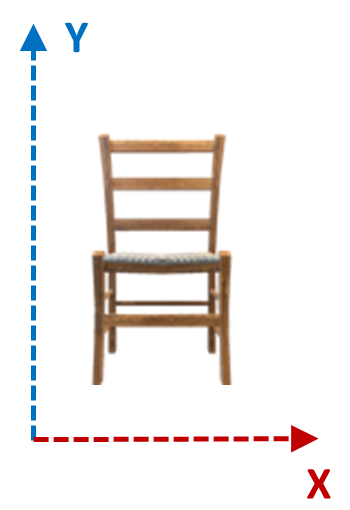
\includegraphics[height=3.5cm]{capitulos/metodos/imagens/chair_front}
        }%
        \hfill
        \subcaptionbox{\label{subfig:our-strategy-3d-side}}{
            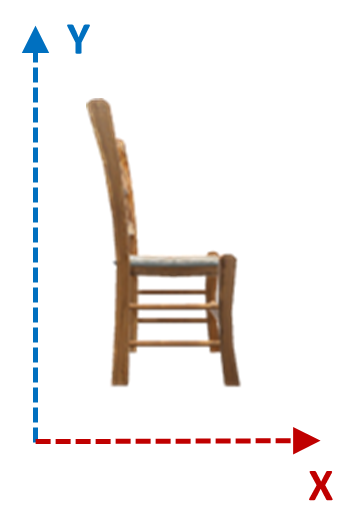
\includegraphics[height=3.5cm]{capitulos/metodos/imagens/chair_side}
        }%
        \hfill
        \subcaptionbox{\label{subfig:our-strategy-3d-persp}}{
            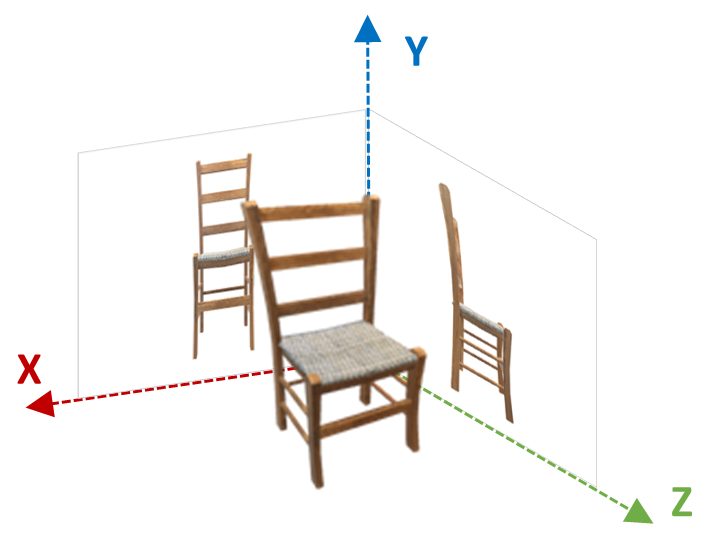
\includegraphics[height=3.5cm]{capitulos/metodos/imagens/chair_perspective}
        }%
    }
    \nomefonte{}
    \label{fig:our-strategy-3d}
\end{figure}


Uma vez definida essa estratégia, nos baseamos no processo descrito por \citeonline{amorim-2019-stgcn-sl} para realizar a estimativa dos esqueletos para os indivíduos nas amostras. Esse processo é composto pelas etapas de obtenção de amostras, segmentação dos sinais, estimativa e normalização dos esqueletos, as quais sofreram adaptações no contexto do presente trabalho para acomodar a composição de esqueletos 3D e os desafios que encontramos para isso. Discutiremos a seguir as adaptações realizadas para superar as limitações dos \textit{datasets} existentes:

% Os passos utilizados para gerar o ASL-Skeleton3D basearam-se no processamento realizado por \citeonline{amorim-2019-stgcn-sl} na construção de um \textit{dataset} de esqueletos 2D da \acrshort{asl}. De um modo geral, eles envolvem a obtenção das amostras, a segmentação dos sinais, a estimativa e a normalização dos esqueletos. Apesar disso, várias adaptações foram necessárias a cada passo para acomodar a estratégia descrita acima e lidar com os desafios encontrados aqui, conforme discutiremos a seguir:

\begin{enumerate}
    \item \textbf{Obtenção das amostras}: nessa etapa as amostras de vídeos são recuperadas a partir dos servidores do \acrshort{asllvd}, mas no contexto atual, fazemos isso para ambas as câmeras frontal e lateral.

          A saber, existem dois formatos nos quais os vídeos dessas câmeras podem ser disponibilizados: o \textit{mov}, que é compacto e mais fácil de processar; e o \textit{.vid}, que consiste no vídeo bruto, que é maior e mais pesado para baixar e processar.
          Ao analisar as amostras, identificamos que parte delas possuía ambas câmeras disponíveis nos dois formatos; para outras, cada câmera estava em um formato distinto; contudo, nos piores casos uma das câmeras estava ausente ou corrompida, fazendo com que essas amostras fossem perdidas. Lidar com essa falta de homogeneidade acrescentou uma complexidade inesperada, mas que foi contornada resultando numa perda de apenas 0,16\% das amostras originais -- ou seja, 16 amostras de um total inicial de 9.763.


    \item \textbf{Segmentação dos sinais}: compreende a segmentação das sequências de vídeos do \acrshort{asllvd} em pedaços menores, contendo um único sinal.
          Nessa etapa também reduzimos a taxa de quadros de 60 para 3 FPS, uma vez que consideramos que é pouco provável a articulação de mais de três movimentos relevantes em um único segundo.
          Isso contribuiu para reduzir em cerca de 20 vezes o número de \textit{frames} a serem processados nas etapas seguintes.


    \item \textbf{Estimativa dos esqueletos 3D}: nesse momento os esqueletos dos sinalizadores são estimados utilizando-se o OpenPose para ambas as câmeras frontal e lateral. Dois esqueletos 2D são obtidos a partir disso:

          \begin{enumerate}
              \item \textit{Esqueleto frontal} (\autoref{subfig:front-side-persp-skeletons-front}), contendo as coordenadas plotadas sobre o eixos \(x\) e \(y\) que correspondem às mesmas coordenadas \(x\) e \(y\) de quando imaginamos o indivíduo representado no espaço tridimensional (vide \autoref{subfig:front-side-persp-skeletons-persp}).
                    % Essas coordenadas descrevem a mesma visão frontal que esperamos obter ao imaginar o nosso esqueleto 3D final observado de frente. Por conta disso, utilizamos essas coordenadas \(x\) e \(y\) da forma como são fornecidas para ancorar o indivíduo no espaço tridimensional. Precisaremos apenas adicionar a dimensão de profundidade.

              \item \textit{Esqueleto lateral} (\autoref{subfig:front-side-persp-skeletons-side}), que também é estimado com um par de coordenadas \(x\) e \(y\) mas que, quando posicionados perpendicularmente ao esqueleto frontal (vide \autoref{subfig:front-side-persp-skeletons-persp}), denotam a dimensão de profundidade e correspondem aos eixos \(z\) e \(y\) do indivíduo no espaço tridimensional, respectivamente. Uma vez que \(y\) já foi obtido por meio do esqueleto frontal, ele pode ser então descartado.

                    % No entanto, vamos aplicar a estratégia descrita acima e posicioná-lo perpendicularmente ao esqueleto frontal (como no ~\autoref{subfig:front-side-persp-skeletons-persp}). Nesse caso, observamos que embora o eixo \(y\) fornecido aqui contenha as mesmas coordenadas que no esqueleto frontal, o eixo \(x\) descreverá coordenadas equivalentes às de profundidade. Dessa forma, tomaremos o eixo \(x\) do esqueleto lateral como sendo o eixo \(z\) (eixo de profundidade) para o nosso esqueleto 3D final.
          \end{enumerate}

          Dessa forma, combinamos as coordenadas \(x\), \(y\) e \(z\) obtidas para dar origem ao nosso esqueleto 3D.

          \begin{figure}[ht!]
              \centering
              \caption{\textmd{Os esqueletos 2D frontal (\subref{subfig:front-side-persp-skeletons-front}) e lateral (\subref{subfig:front-side-persp-skeletons-side}) são posicionados perpendicularmente (\subref{subfig:front-side-persp-skeletons-persp}) e combinados para compor o esqueleto 3D final utilizado aqui}}
              \borda[0.85\textwidth]{
                  \subcaptionbox{\label{subfig:front-side-persp-skeletons-front}}{
                      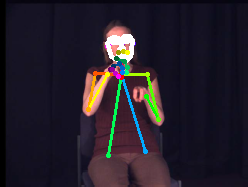
\includegraphics[height=2.5cm]{capitulos/metodos/imagens/asllvd_example_front_skeleton}
                  }%
                  \hfill
                  \subcaptionbox{\label{subfig:front-side-persp-skeletons-side}}{
                      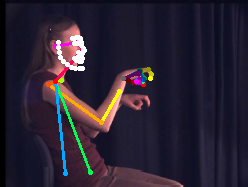
\includegraphics[height=2.5cm]{capitulos/metodos/imagens/asllvd_example_side_skeleton}
                  }%
                  \hfill
                  \subcaptionbox{\label{subfig:front-side-persp-skeletons-persp}}{
                      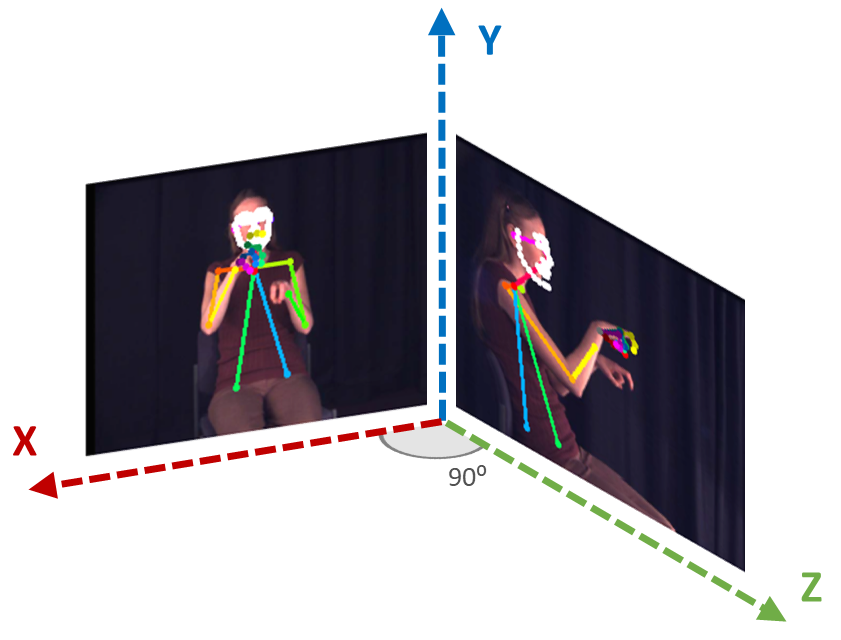
\includegraphics[height=4.0cm]{capitulos/metodos/imagens/asllvd_front_side_perspective_skeleton}
                  }%
              }
              \nomefonte{}
              \label{fig:front-side-persp-skeletons}
          \end{figure}


    \item \textbf{Normalização dos esqueletos 3D}: por fim, os esqueletos 3D são normalizados para remover variações decorrentes do posicionamento das câmeras e dos corpos dos indivíduos. Isso é importante porque o \acrshort{asllvd} foi capturado através de diferentes seções e envolveu diferentes sinalizadores.

          Adotamos como referência para essa normalização a largura entre os ombros dos sinalizadores (vide \autoref{fig:shoulders-width}), a qual foi inspirada pela medida antropométrica de \textit{diâmetro biacromial} apresentada por \citeonline{stoudt-1970-skinfolds}. Dessa forma, a largura entre os ombros \(W_{shoulders}\) é definida aqui como a distância euclidiana \(d\) entre as coordenadas do ombro esquerdo \(S_{l}\) e do ombro direito \(S_ {r}\), conforme \autoref{eqn:shoulders-width}:

          \figura
          {fig:shoulders-width} % Label
          {capitulos/metodos/imagens/shoulders_width} % Path
          {height=3.5cm} % Size
          {A largura entre ombros foi utilizada para normalizar as coordenadas nos esqueletos 3D} % Caption
          {} % Citation

          \begin{equation}
              \label{eqn:shoulders-width}
              W_{shoulders} = d\left(S_{l}, S_{r}\right)
          \end{equation}

          Utilizando-se \(W_{shoulders}\) é possível transformar as coordenadas \(K\) do esqueleto 3D em coordenadas normalizadas \(K_{norm}\), conforme \autoref{eqn:normalized-keypoint}:

          % Normalização de pontos-chave:
          \begin{equation}
              \label{eqn:normalized-keypoint}
              K_{norm} = \frac{K}{W_{shoulders}}
          \end{equation}

\end{enumerate}


A \autoref{fig:sample-json-datasetTD} exemplifica uma amostra do ASL-Skeleton3D resultante do processamento acima, bem como suas propriedades. Observa-se no início do arquivo informações básicas extraídas do \acrshort{asllvd}, como rótulo, nome do indivíduo, sessão, cena, \textit{frames} de início e fim, entre outras. Na propriedade ``\textit{frames}'' estão listados os \textit{frames} para aquela sequência e o esqueleto 3D estimado para cada um deles. Cada esqueleto contém grupos referentes ao ``\textit{body}'' (corpo), ``\textit{face}'' (face), ``\textit{hand left}'' (mão esquerda) e ``\textit{hand right}'' (mão direita) que, por sua vez, contêm propriedades que listam o nome da coordenada, o ``\textit{score}'' (ou acurácia) de sua estimativa e os respectivos eixos \(x\), \(y\) e \(z\).
Por exemplo, se observarmos o primeiro índice das propriedades do grupo ``\textit{body}'' veremos que ele corresponde à coordenada ``\textit{nose}'' (nariz), apresenta um \textit{score} de aproximadamente 90\% e coordenadas \(x\), \(y\) e \(z\) localizadas em 4,488, 1,696 e 2,872.

\figura
{fig:sample-json-datasetTD} % Label
{capitulos/metodos/imagens/code_3d} % Path
{width=0.7\linewidth} % Size
{Exemplo de amostra do ASL-Skeleton3D} % Caption
{} % Citation

O \textit{dataset} final e o código-fonte utilizado para o processamento apresentado nesta seção estão disponíveis publicamente na URL listada abaixo\footnote{Disponível em \url{http://www.cin.ufpe.br/~cca5/asl-skeleton3d}}.


% Dataset phono
\subsection{ASL-Phono}
\label{sec:metodos-datasets-phono}

O ASL-Phono é um \textit{dataset} que introduz uma representação baseada na linguística da língua de sinais e a descreve em termos de seus atributos fonológicos. 
Ele é produzido a partir dos esqueletos fornecidos pelo \textit{dataset} ASL-Skeleton3D e, assim como este, também apresenta 9.747 amostras correspondentes a 2.650 sinais distintos. 
Além disso, a abordagem utilizada para computar esses atributos pode ser replicada para outras línguas de sinais.

Por se tratar de uma versão inicial da representação proposta, neste trabalho será selecionado apenas um subconjunto dos parâmetros fonológicos introduzidos na \autoref{sec:linguistica} para que, dessa forma, seja possível validar sua efetividade e traçar uma direção para iterações futuras.
Sendo assim, descrevem-se a seguir esses parâmetros, bem como a estratégia utilizada para calculá-los e representá-los computacionalmente:

\begin{enumerate}
    \item \textbf{Configuração de mão}: é a configuração de mão utilizada pelo sinalizador na articulação do sinal.

          O \acrshort{asllvd} fornece originalmente as configurações de mão inicial e final para cada sinal, descrita de acordo com as 88 opções apresentadas por \citeonline{neidle-2020-asllrp} no \acrfull{asllrp}\footnote{
              Disponível em \url{http://www.bu.edu/asllrp}
          }.
          Foi utilizada essa mesma informação para o ASL-Phono, porém adicionou-se um passo extra para distribuir essas configurações entre todos os \textit{frames}, e não apenas o inicial e final.
          Dessa forma, dividiu-se a sequência de \textit{frames} em duas metades e associou-se à primeira delas a configuração inicial provida pelo \acrshort{asllvd} e, à segunda, a configuração final.

    \item \textbf{Orientação}: é a direção apontada pelas palmas das mãos na articulação dos sinais.

          Para calculá-la, foi utilizada álgebra linear para explorar a relação das mãos com o espaço tridimensional em que suas coordenadas estão inseridas.
          Primeiramente, assumiu-se que cada palma é um plano cartesiano que atravessa as coordenadas estimadas para as mãos (vide \autoref{subfig:palm-orientation}). Selecionaram-se então três dessas coordenadas para descrever o plano: \(W\), que corresponde à coordenada do pulso; \(L\), localizada na base do dedo mínimo; e \(I\), localizada na base do dedo indicador.

          \begin{figure}[ht!]
              \centering
              \caption{
                  \textmd{
                      As coordenadas \(W\), \(L\) e \(I\) são utilizados para obter a normal \(\protect \overrightarrow{n}\) da palma da mão~(\subref{subfig:palm-orientation}), a qual é utilizada para calcular a orientação da palma \(O_{palm}\)~(\subref{subfig:palm-directions})
                  }
              }
              \borda[0.60\textwidth]{
                  \subcaptionbox{\label{subfig:palm-orientation}}{
                      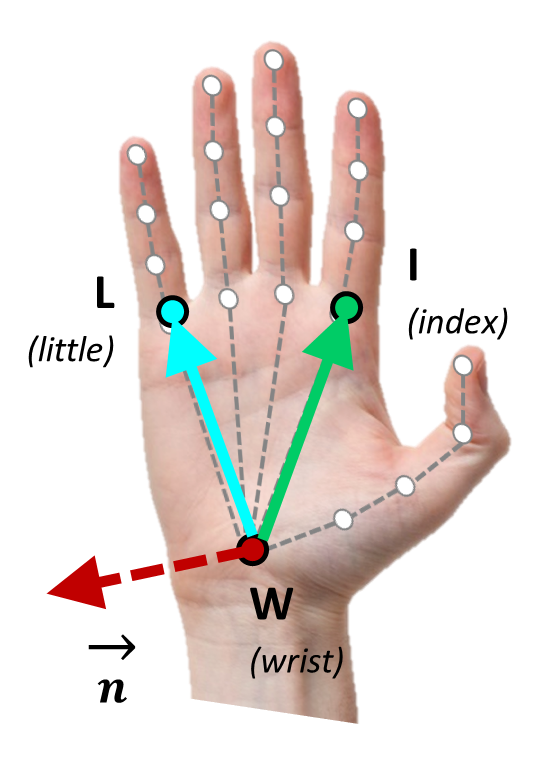
\includegraphics[height=3.8cm]{capitulos/metodos/imagens/palm_orientation_algebra}
                  }%
                  \hfill
                  \subcaptionbox{\label{subfig:palm-directions}}{
                      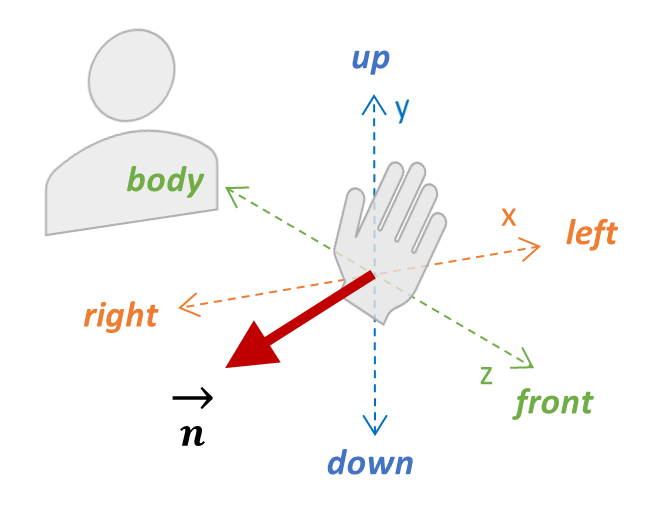
\includegraphics[height=4cm]{capitulos/metodos/imagens/hand_orientations}
                  }%
              }
              \nomefonte{}
              \label{fig:palm-orientation-directions}
          \end{figure}

          A partir dessas coordenadas, \citeonline{anton-2013-algebra} afirmam que pode-se estabelecer dois vetores auxiliares em termos dos quais esse mesmo plano cartesiano também é descrito (vide \autoref{subfig:palm-orientation}): \(\overrightarrow{WL}\), indicado pela seta azul e \(\overrightarrow{WI}\), indicado pela seta verde.
          Por meio deles, calculou-se o vetor normal \(\overrightarrow{n}\) utilizando a \autoref{eqn:normal-palm-left} (para a mão esquerda) e \autoref{eqn:normal-palm-right} (para a mão direita). \(\overrightarrow{n}\), que é perpendicular à palma da mão, é ilustrado na \autoref{subfig:palm-orientation} como uma seta tracejada vermelha.

          % Palm orientation:
          \begin{equation}
              \label{eqn:normal-palm-left}
              \overrightarrow{n}_{left} = \overrightarrow{WI} \times \overrightarrow{WL}
          \end{equation}

          \begin{equation}
              \label{eqn:normal-palm-right}
              \overrightarrow{n}_{right} = \overrightarrow{WL} \times \overrightarrow{WI}
          \end{equation}

          Por fim, utilizou-se os valores das coordenadas de \(\overrightarrow{n}\) para definir a orientação da palma \(O_{palm}\), conforme \autoref{eqn:palm-orientation-directions}.
          Essa orientação consiste na combinação de até três das seguintes direções: \textit{right} (direita), \textit{left} (esquerda), \textit{up} (para cima), \textit{down} (para baixo), \textit{body} (voltada para o corpo) ou \textit{front} (para frente).
          Por exemplo, ``\textit{right\_front\_down}'' seria uma orientação válida indicando que a palma da mão está inclinada, conforme ilustrado na \autoref{subfig:palm-directions}.

          % Directions
          \begin{equation}
              \label{eqn:palm-orientation-directions}
              O_{palm} =
              \begin{cases}
                  right & \text{if $\overrightarrow{n}_x < {-k}$ } \\
                  left  & \text{if $\overrightarrow{n}_x > {k}$ }  \\
                  up    & \text{if $\overrightarrow{n}_y < {-k}$ } \\
                  down  & \text{if $\overrightarrow{n}_y > {k}$ }  \\
                  body  & \text{if $\overrightarrow{n}_z < {-k}$ } \\
                  front & \text{if $\overrightarrow{n}_z > {k}$ }  \\
              \end{cases}
          \end{equation}

          Na \autoref{eqn:palm-orientation-directions}, \(k\) é definido empiricamente como 0,30 para filtrar variações pouco significativas em \(\overrightarrow{n}\).


    \item \textbf{Movimento}: é o deslocamento realizado pelas mãos na articulação do sinal.

          Para calculá-lo, primeiro será selecionada como referência a coordenada \(M\) localizada na base do dedo médio (vide \autoref{subfig:hand-movement}).
          Em seguida, será obtido seu deslocamento entre os \textit{frames} anterior (tempo \(t-1\)) e atual (tempo \(t\)) utilizando a \autoref{eqn:hand-movement} que, por sua vez, fornecerá o vetor de movimento \(\overrightarrow{m}\) (indicado pela seta tracejada vermelha na \autoref{subfig:hand-movement}).

          \begin{figure}[ht!]
              \centering
              \caption{
                  \textmd{
                      O vetor de movimento \(\protect \overrightarrow{m}\) é obtido através da trajetória da coordenada \(M\) entre os frames anterior (\(t-1\)) e atual (\(t\))~(\subref{subfig:hand-movement}); \(\protect \overrightarrow{m}\) é então utilizado para calcular o movimento da mão \(V_{hand}\)~(\subref{subfig:hand-directions})
                  }
              }
              \borda[0.7\textwidth]{
                  \subcaptionbox{\label{subfig:hand-movement}}{
                      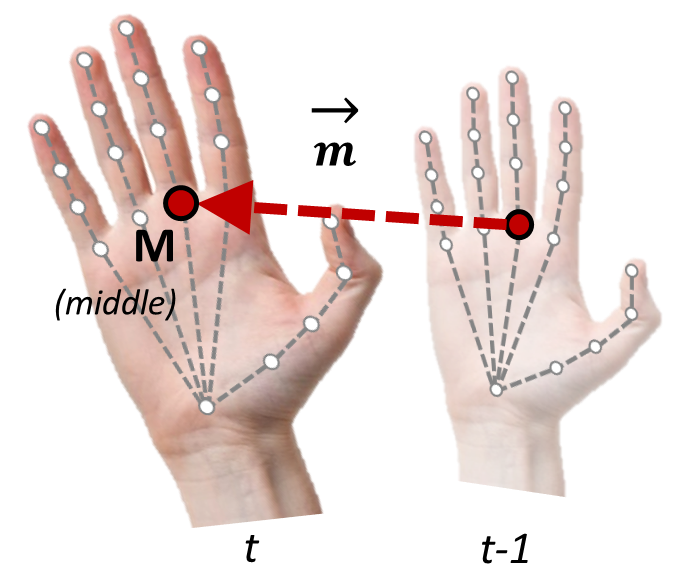
\includegraphics[height=3.5cm]{capitulos/metodos/imagens/hand_movement}
                  }%
                  \hfill
                  \subcaptionbox{\label{subfig:hand-directions}}{
                      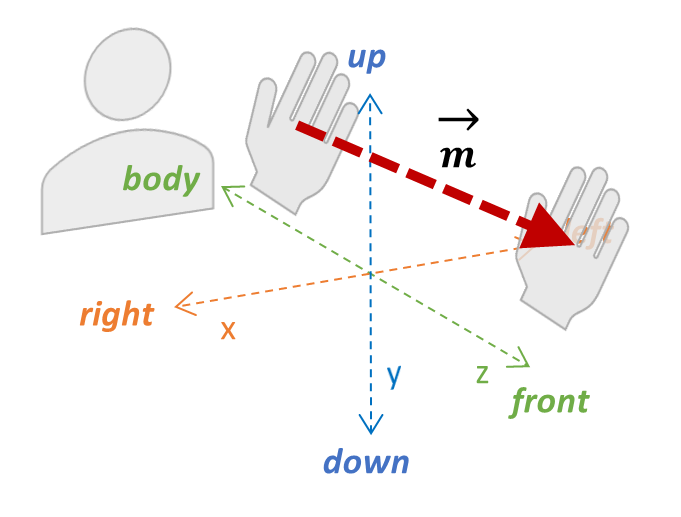
\includegraphics[height=4cm]{capitulos/metodos/imagens/hand_movement_2}
                  }%
              }
              \nomefonte{}
              \label{fig:hand-movement-directions}
          \end{figure}

          % Movement of the hands:
          \begin{equation}
              \label{eqn:hand-movement}
              \overrightarrow{m} = M_{t} - M_{t-1}
          \end{equation}

          A partir de \(\overrightarrow{m}\), pode-se então calcular o movimento da mão \(V_{hand}\) através da \autoref{eqn:hand-movement-directions}, que consiste numa operação semelhante àquela utilizada para a orientação da mão.
          Com isso, \(V_{hand}\) também consistirá na combinação de até três direções: \textit{right} (direita), \textit{left} (esquerda), \textit{up} (para cima), \textit{down} (para baixo), \textit{body} (para o corpo) ou \textit{front} (para frente).
          A \autoref{subfig:hand-directions} ilustra um movimento categorizado com a direção ``\textit{front}''.

          % Directions
          \begin{equation}
              \label{eqn:hand-movement-directions}
              V_{hand} =
              \begin{cases}
                  right & \text{if $\overrightarrow{m}_x < {-k}$ } \\
                  left  & \text{if $\overrightarrow{m}_x > {k}$ }  \\
                  up    & \text{if $\overrightarrow{m}_y < {-k}$ } \\
                  down  & \text{if $\overrightarrow{m}_y > {k}$ }  \\
                  body  & \text{if $\overrightarrow{m}_z < {-k}$ } \\
                  front & \text{if $\overrightarrow{m}_z > {k}$ }  \\
              \end{cases}
          \end{equation}

          Na \autoref{eqn:hand-movement-directions} o limiar \(k\) foi também estabelecido empiricamente como 0,30, para filtrar movimentos com baixa relevância.


    \item \textbf{Expressão não-manual (abertura da boca)}: captura o grau de abertura da boca para cada \textit{frame} na articulação do sinal que, por sua vez, denota a existência de expressão não-manual envolvendo ela.

          Para computar essa \textit{feature}, utilizou-se como referência o trabalho de \citeonline{ferrario-2000-study-lips}, que analisa e propõe medidas antropométricas para os lábios.
          Dentre elas, foi selecionada a \textit{vermilion height to mouth width} (ou altura dos lábios com relação à largura da boca) para estabelecer a abertura da boca \(P_{mouth}\), uma vez que essa medida é capaz de capturar a proporção de abertura dos lábios em termos de um único número.
          A \autoref{eqn:mouth-openness} define formalmente o cálculo de \(P_{mouth}\), que consiste na proporção entre a altura e a largura dos lábios:

          % Abertura da boca:
          \begin{equation}
              \label{eqn:mouth-openness}
              P_{mouth} = \frac{d(LS, LI)}{d(CH_r, CH_l)}
          \end{equation}

          A altura dos lábios é dada pela distância \(d\) entre as coordenadas do \textit{labiale superius} \(LS\) e do \textit{labiale inferius} \(LI\), que são os pontos mais externos aos lábios superior e inferior, respectivamente. A largura, por sua vez, consiste na distância entre as coordenadas do \textit{cheilion} direito \(CH_r\) e do \textit{cheilion} esquerdo \(CH_l\), que são os pontos situados nos cantos direito e esquerdo dos lábios, conforme ilustra a \autoref{fig:mouth-openness}.

          \figura
          {fig:mouth-openness} % Label
          {capitulos/metodos/imagens/mouth_openness} % Path
          {height=3.5cm} % Size
          {A abertura da boca \(P_{mouth}\) é obtida a partir da medida antropométrica \textit{vermilion height to mouth width} que utiliza quatro coordenadas dos lábios para calcular uma única proporção} % Caption
          {ferrario-2000-study-lips} % Citation

\end{enumerate}


Essas são as \textit{features} extraídas para o ASL-Phono.
O \autoref{cod:sample-json-phono} exemplifica uma amostra resultante desse processo, bem como a disposição dos atributos fonológicos em suas propriedades.
Atributos com sufixo ``dh'' referem-se à \textit{dominant hand} (mão dominante) e aqueles com ``ndh'' referem-se à \textit{non-dominant hand} (mão não-dominante).
Sua estrutura é muito semelhante àquela apresentada para o ASL-Skeleton3D, exceto pela propriedade ``\textit{frames}'' que, ao invés de coordenadas 3D, aqui contém os atributos computados acima.
Além do seu respectivo valor computado, cada atributo pode apresentar também um \textit{score}, que é obtido a partir da precisão estimada para as coordenadas envolvidas no seu cálculo.

\codigo
    {cod:sample-json-phono}
    {capitulos/metodos/codigos/exemplo_phono.m}
    {ASLDataset}
    {Exemplo de amostra do \textit{dataset} ASL-Phono}
    {}



% Estatísticas:
A \autoref{tab:dataset-phono-stats}, por sua vez, apresenta estatísticas calculadas para o \textit{dataset} resultante que nos fornecem um panorama da distribuição final de suas amostras, bem como do número de movimentos, orientações, configurações de mão e variação na abertura de boca computados acima.

% Please add the following required packages to your document preamble:
% \usepackage{multirow}
% \usepackage{graphicx}
% \usepackage[table,xcdraw]{xcolor}
% If you use beamer only pass "xcolor=table" option, i.e. \documentclass[xcolor=table]{beamer}
\begin{table}[ht!]
    \centering
    \caption{Estatísticas calculadas a partir do ASL-Phono, as quais são visualizadas para todo o \textit{dataset} e segundo agrupamentos por amostra e por sinal. (D) refere-se à mão dominante e (ND) refere-se à mão não-dominante}
    \label{tab:dataset-phono-stats}
    \resizebox{0.9\textwidth}{!}{%
        \begin{tabular}{cr|ccc|ccccccc}
            \hline
            \rowcolor[HTML]{EFEFEF}
                                                                                     &        & \cellcolor[HTML]{EFEFEF}                           & \cellcolor[HTML]{EFEFEF}                         & \cellcolor[HTML]{EFEFEF}                         & \multicolumn{2}{c}{\cellcolor[HTML]{EFEFEF}Movimento} & \multicolumn{2}{c}{\cellcolor[HTML]{EFEFEF}Orientação} & \multicolumn{2}{c}{\cellcolor[HTML]{EFEFEF}Config. mão} & \cellcolor[HTML]{EFEFEF}                                                                                                                       \\
            \rowcolor[HTML]{EFEFEF}
                                                                                     &        & \multirow{-2}{*}{\cellcolor[HTML]{EFEFEF}Nº amostras} & \multirow{-2}{*}{\cellcolor[HTML]{EFEFEF}Nº sinais} & \multirow{-2}{*}{\cellcolor[HTML]{EFEFEF}Nº frames} & (D)                                                   & (ND)                                                   & (D)                                                     & (ND)                     & (D)  & (ND) & \multirow{-2}{*}{\cellcolor[HTML]{EFEFEF}\begin{tabular}[c]{@{}c@{}}Abertura \\ da boca\end{tabular}} \\ \hline
            \begin{tabular}[c]{@{}c@{}}\textit{Dataset}\end{tabular}      & Total  & 9.747                                              & 2.650                                            & -                                                & 26                                                    & 26                                                     & 26                                                      & 26                       & 85   & 78   & -                                                                                                     \\ \hline
                                                                                     & Mín    & -                                                  & -                                                & 1                                                & 0                                                     & 0                                                      & 0                                                       & 0                        & 0    & 0    & 0,01                                                                                                  \\
                                                                                     & Máx    & -                                                  & -                                                & 12                                               & 10                                                    & 8                                                      & 6                                                       & 5                        & 2    & 2    & 2,19                                                                                                  \\
                                                                                     & Média  & -                                                  & -                                                & 3,02                                             & 1,94                                                  & 1,26                                                   & 2,20                                                    & 1,18                     & 1,17 & 0,72 & 0,13                                                                                                  \\
            \multirow{-4}{*}{\begin{tabular}[c]{@{}c@{}}Por \\ amostra\end{tabular}} & Desvio & -                                                  & -                                                & 0,87                                             & 0,83                                                  & 1,15                                                   & 0,79                                                    & 1,07                     & 0,38 & 0,58 & 0,12                                                                                                  \\ \hline
                                                                                     & Mín    & 1                                                  & -                                                & -                                                & 1                                                     & 0                                                      & 1                                                       & 0                        & 1    & 0    & 0,02                                                                                                  \\
                                                                                     & Máx    & 59                                                 & -                                                & -                                                & 24                                                    & 16                                                     & 22                                                      & 14                       & 8    & 8    & 0,99                                                                                                  \\
                                                                                     & Média  & 3,68                                               & -                                                & -                                                & 6,04                                                  & 3,66                                                   & 5,37                                                    & 2,63                     & 1,81 & 1,17 & 0,13                                                                                                  \\
            \multirow{-4}{*}{\begin{tabular}[c]{@{}c@{}}Por \\ sinal\end{tabular}}   & Desvio & 2,67                                               & -                                                & -                                                & 2,93                                                  & 3,18                                                   & 2,29                                                    & 2,35                     & 0,99 & 1,14 & 0,07                                                                                                  \\ \hline
        \end{tabular}%
    }
    \nomefonte{}
\end{table}

Existem três agrupamentos contidos nessa tabela:

\begin{itemize}
    \item \textit{Dataset}: sumariza o total de amostras, de sinais e de cada um dos atributos computados para o \textit{dataset}.
          Por exemplo, há um total de 9.747 amostras e 26 movimentos possíveis para a mão dominante.

    \item Por amostra: fornece estatísticas de mínimo, máximo, média e desvio padrão calculadas agrupando-se o \textit{dataset} por amostra.
          Por exemplo, há em média 3,02 \textit{frames} por amostra e esse número varia de 1 a 12 \textit{frames}; de maneira semelhante, as amostras têm em média 1,94 movimentos distintos para a mão dominante, o que varia entre 0 e 10 movimentos.

    \item Por sinal: fornece estatísticas de mínimo, máximo, média e desvio padrão calculadas agrupado-se o \textit{dataset} por sinal.
          Por exemplo, cada sinal tem em média 3,68 amostras e isso pode variar de 1 até 59 -- no entanto, o desvio padrão nos revela que tal variação concentra-se muito mais em torno da média; nota-se também que a mão dominante realiza em média 6,04 movimentos distintos em um único sinal, o que pode variar de 1 a 24 para outros.

\end{itemize}


Por fim, a \autoref{fig:dataset-resampling-antes} detalha a relação entre o número de sinais e o número de amostras existentes no ASL-Phono. Por meio desta análise, percebe-se mais claramente que a maior parte dos sinais concentra-se na faixa de 1 e 6 amostras, que é exatamente o intervalo descrito pela média e desvio padrão da tabela acima.
No entanto, há sinais que apresentam 7 ou mais amostras e ainda outros casos atípicos em que 1, 2 ou 3 sinais que concentram sozinhos um número muito grande de amostras -- de 13 até 59.
Será discutida na seção seguinte a abordagem utilizada neste trabalho para lidar com esse desbalanceamento e homogeneizar as amostras antes de prosseguir com os experimentos.

\figura
{fig:dataset-resampling-antes} % Label
{capitulos/metodos/imagens/dataset_resampling_antes} % Path
{height=5.5cm} % Size
{Relação entre número de sinais e número de amostras disponíveis no ASL-Phono} % Caption
{} % Citation


O \textit{dataset} e o código-fonte resultantes do processamento apresentado nesta seção estão disponíveis publicamente na URL listada abaixo\footnote{Disponível em \url{http://www.cin.ufpe.br/~cca5/asl-phono}}.

